\subsection{COVID-19 Data}
\paragraph{Calculating the severity of COVID-19}

Since the purpose of this project is to investigate the correlation between COVID-19 pandemic and  $CO_2$ emissions, we needed a dataset, that provides recent and detailed information on COVID-19 statistics per country. These necessary statistics include number of cases, deaths and recoveries. Accessibility, detail and up-to-dateness of Bing COVID-19 dataset \cite{Bing} made it our primary choice for getting COVID statistics.

Eventually we will need to compare the change in $CO_2$ emissions against the severity of COVID-19 cases in a given country. Since the values in Bing database are absolute, we also need population data for each country. After we combined population information, extracted from \cite{PopulationData}, with COVID-19 statistics, we were able to calculate the severity of COVID-19 in any given country, i.e. deaths and cases per 100,000 people. These rates are visualized in \autoref{fig:covidimpact}. This information is to be compared and correlated with predicted $CO_2$ emissions.

\begin{figure}[h]
	\centering
	\begin{subfigure}[b]{0.47\linewidth}
		\includegraphics[width=\linewidth]{../covid/case rate}
	\end{subfigure}
	\begin{subfigure}[b]{0.47\linewidth}
		\includegraphics[width=\linewidth]{../covid/death rate}
	\end{subfigure}
	\caption{Covid-19 rates for each country.}
	\label{fig:covidimpact}
\end{figure}


\begin{figure}[h]
	\centering
	\begin{subfigure}[b]{0.47\linewidth}
		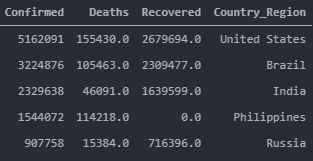
\includegraphics[width=\linewidth]{../covid/bing_top5}
	\end{subfigure}
	\caption{5 countries which have the highest number of cases.}
	\label{fig:bingtop5}
\end{figure}